\begin{frame}
	\frametitle{Procedimento 02}
	\framesubtitle{Descrição}
	\only<1>{
		\begin{itemize}
			\item 300 testes aleatórios em cada caso.
			\item EER = equilibrio entre as taxas de falsos positivos e de falsos negativos.
			\item Em alguns casos o cálculo do EER necessitou mais iterações.
			\item 10\%, 20\%, 30\%, 40\% e 50\% da base de sinais reservados para treinamento.
		\end{itemize}
	}	
\end{frame}
	
\begin{frame}[allowframebreaks]
	\frametitle{Procedimento 02}
		\framesubtitle{Tabelas de resultados}
		\begin{table}[h]
	\newcommand{\mc}[3]{\multicolumn{#1}{#2}{#3}}
	\definecolor{tcA}{rgb}{0.65098,0.65098,0.65098}
	\definecolor{tcB}{rgb}{0.447059,0.74902,0.266667}
	\begin{center}
		\begin{tabular}{|l|l|l|}\hline
			% use packages: color,colortbl
			\rowcolor{tcA}
			\textbf{Tamanho do modelo} & \textbf{Acurácia mínima} & \textbf{Acurácia máxima}\\\hline
			\rowcolor{tcB}
			\mc{1}{|c|}{10\%} & \mc{1}{c|}{0,6666} & \mc{1}{c|}{0,8861}\\\hline
			\rowcolor{tcB}
			\mc{1}{|c|}{20\%} & \mc{1}{c|}{0,7439} & \mc{1}{c|}{0,8902}\\\hline
			\rowcolor{tcB}
			\mc{1}{|c|}{30\%} & \mc{1}{c|}{0,7665} & \mc{1}{c|}{0,8919}\\\hline
			\rowcolor{tcB}
			\mc{1}{|c|}{40\%} & \mc{1}{c|}{0,7784} & \mc{1}{c|}{0,9024}\\\hline
			\rowcolor{tcB}
			\mc{1}{|c|}{50\%} & \mc{1}{c|}{0,7804} & \mc{1}{c|}{0,9097}\\\hline
		\end{tabular}
	\end{center}
	\caption{Resultados do experimento 02}
	\label{tab:experiment02Results}
\end{table}
\end{frame}

\begin{frame}[allowframebreaks]
	\frametitle{Procedimento 02}
		\framesubtitle{Tabelas de confusão}
		\begin{table}[H] 					\newcommand{\mc}[3]{\multicolumn{#1}{#2}{#3}} 					\definecolor{tcB}{rgb}{0.447059,0.74902,0.266667} 					\definecolor{tcC}{rgb}{0,0,0} 					\definecolor{tcD}{rgb}{0,0.5,1} 					\definecolor{tcA}{rgb}{0.65098,0.65098,0.65098} 					\begin{center} 						\subfloat[Melhor matriz de confusão]{ 							\begin{tabular}{ccc} 								\mc{1}{l}{} & \mc{1}{>{\columncolor{tcA}}c}{\textbf{genuíno}} & \mc{1}{>{\columncolor{tcA}}c}{\textbf{falseado}}\\ 								\mc{1}{>{\columncolor{tcA}}r}{\textbf{genuíno}} & \mc{1}{>{\columncolor{tcB}}c}{\textcolor{tcC}{363}} & \mc{1}{>{\columncolor{tcD}}c}{\textcolor{tcC}{14}}\\ 								\mc{1}{>{\columncolor{tcA}}r}{\textbf{falseado}} & \mc{1}{>{\columncolor{tcD}}c}{\textcolor{tcC}{6}} & \mc{1}{>{\columncolor{tcB}}c}{\textcolor{tcC}{355}} 							\end{tabular} 							\label{tab:classifier_Euclidian_10_best} 						} 						\qquad 						\subfloat[Pior matriz de confusão]{ 							\begin{tabular}{ccc} 								\mc{1}{l}{} & \mc{1}{>{\columncolor{tcA}}c}{\textbf{genuíno}} & \mc{1}{>{\columncolor{tcA}}c}{\textbf{falseado}}\\ 								\mc{1}{>{\columncolor{tcA}}r}{\textbf{genuíno}} & \mc{1}{>{\columncolor{tcB}}c}{\textcolor{tcC}{275}} & \mc{1}{>{\columncolor{tcD}}c}{\textcolor{tcC}{10}}\\ 								\mc{1}{>{\columncolor{tcA}}r}{\textbf{falseado}} & \mc{1}{>{\columncolor{tcD}}c}{\textcolor{tcC}{94}} & \mc{1}{>{\columncolor{tcB}}c}{\textcolor{tcC}{359}} 							\end{tabular} 							\label{tab:classifier_Euclidian_10_worse} 						} 					\end{center} 					\caption{Matrizes de confusão para distância Euclidiana com modelo a 10\%} 				\end{table}
		\begin{table}[h]
\newcommand{\mc}[3]{\multicolumn{#1}{#2}{#3}}
\definecolor{tcB}{rgb}{0.447059,0.74902,0.266667}
\definecolor{tcC}{rgb}{0,0,0}
\definecolor{tcD}{rgb}{0,0.4,0.701961}
\definecolor{tcA}{rgb}{0.65098,0.65098,0.65098}
\begin{center}
	\begin{tabular}{ccc}
		% use packages: color,colortbl
		\mc{1}{l}{} & \mc{1}{>{\columncolor{tcA}}c}{\textbf{genuíno}} & \mc{1}{>{\columncolor{tcA}}c}{\textbf{regravado}}\\

		\mc{1}{>{\columncolor{tcA}}r}{\textbf{genuíno}} & \mc{1}{>{\columncolor{tcB}}c}{\textcolor{tcC}{308}} & \mc{1}{>{\columncolor{tcD}}c}{\textcolor{tcC}{50}}\\

		\mc{1}{>{\columncolor{tcA}}r}{\textbf{regravado}} & \mc{1}{>{\columncolor{tcD}}c}{\textcolor{tcC}{20}} & \mc{1}{>{\columncolor{tcB}}c}{\textcolor{tcC}{278}}
	\end{tabular}
	\caption{Melhor matriz de confusão para o classificador por distâncias Euclidianas com o uso de 20\% da base para modelagem}
	\label{tab:classifier_Euclidian_20_best}
\end{center}
\end{table}

\begin{table}[h]
	\newcommand{\mc}[3]{\multicolumn{#1}{#2}{#3}}
	\definecolor{tcB}{rgb}{0.447059,0.74902,0.266667}
	\definecolor{tcC}{rgb}{0,0,0}
	\definecolor{tcD}{rgb}{0,0.4,0.701961}
	\definecolor{tcA}{rgb}{0.65098,0.65098,0.65098}
	\begin{center}
		\begin{tabular}{ccc}
			% use packages: color,colortbl
			\mc{1}{l}{} & \mc{1}{>{\columncolor{tcA}}c}{\textbf{genuíno}} & \mc{1}{>{\columncolor{tcA}}c}{\textbf{regravado}}\\
			
			\mc{1}{>{\columncolor{tcA}}r}{\textbf{genuíno}} & \mc{1}{>{\columncolor{tcB}}c}{\textcolor{tcC}{295}} & \mc{1}{>{\columncolor{tcD}}c}{\textcolor{tcC}{137}}\\
			
			\mc{1}{>{\columncolor{tcA}}r}{\textbf{regravado}} & \mc{1}{>{\columncolor{tcD}}c}{\textcolor{tcC}{33}} & \mc{1}{>{\columncolor{tcB}}c}{\textcolor{tcC}{191}}
		\end{tabular}
		\caption{Pior matriz de confusão para o classificador por distâncias Euclidianas com o uso de 20\% da base para modelagem}
		\label{tab:classifier_Euclidian_20_worse}
	\end{center}
\end{table}

		\begin{table}[H] 					\newcommand{\mc}[3]{\multicolumn{#1}{#2}{#3}} 					\definecolor{tcB}{rgb}{0.447059,0.74902,0.266667} 					\definecolor{tcC}{rgb}{0,0,0} 					\definecolor{tcD}{rgb}{0,0.5,1} 					\definecolor{tcA}{rgb}{0.65098,0.65098,0.65098} 					\begin{center} 		\caption{Matrizes de confusão para distância Euclidiana com modelo a 30\%}				\subfloat[Melhor matriz de confusão]{ 							\begin{tabular}{ccc} 								\mc{1}{l}{} & \mc{1}{>{\columncolor{tcA}}c}{\textbf{genuíno}} & \mc{1}{>{\columncolor{tcA}}c}{\textbf{falseado}}\\ 								\mc{1}{>{\columncolor{tcA}}r}{\textbf{genuíno}} & \mc{1}{>{\columncolor{tcB}}c}{\textcolor{tcC}{283}} & \mc{1}{>{\columncolor{tcD}}c}{\textcolor{tcC}{8}}\\ 								\mc{1}{>{\columncolor{tcA}}r}{\textbf{falseado}} & \mc{1}{>{\columncolor{tcD}}c}{\textcolor{tcC}{4}} & \mc{1}{>{\columncolor{tcB}}c}{\textcolor{tcC}{279}} 							\end{tabular} 							\label{tab:classifier_Euclidian_30_best} 						} 						\qquad 						\subfloat[Pior matriz de confusão]{ 							\begin{tabular}{ccc} 								\mc{1}{l}{} & \mc{1}{>{\columncolor{tcA}}c}{\textbf{genuíno}} & \mc{1}{>{\columncolor{tcA}}c}{\textbf{falseado}}\\ 								\mc{1}{>{\columncolor{tcA}}r}{\textbf{genuíno}} & \mc{1}{>{\columncolor{tcB}}c}{\textcolor{tcC}{258}} & \mc{1}{>{\columncolor{tcD}}c}{\textcolor{tcC}{20}}\\ 								\mc{1}{>{\columncolor{tcA}}r}{\textbf{falseado}} & \mc{1}{>{\columncolor{tcD}}c}{\textcolor{tcC}{29}} & \mc{1}{>{\columncolor{tcB}}c}{\textcolor{tcC}{267}} 							\end{tabular} 							\label{tab:classifier_Euclidian_30_worse} 						} 					\\Fonte: Elaborado pelo autor, 2021.		\end{center} 					 				\end{table}
		\begin{table}[h]
\newcommand{\mc}[3]{\multicolumn{#1}{#2}{#3}}
\definecolor{tcB}{rgb}{0.447059,0.74902,0.266667}
\definecolor{tcC}{rgb}{0,0,0}
\definecolor{tcD}{rgb}{0,0.4,0.701961}
\definecolor{tcA}{rgb}{0.65098,0.65098,0.65098}
\begin{center}
	\begin{tabular}{ccc}
		% use packages: color,colortbl
		\mc{1}{l}{} & \mc{1}{>{\columncolor{tcA}}c}{\textbf{Verdadeiro}} & \mc{1}{>{\columncolor{tcA}}c}{\textbf{Falso}}\\

		\mc{1}{>{\columncolor{tcA}}r}{\textbf{Verdadeiro}} & \mc{1}{>{\columncolor{tcB}}c}{\textcolor{tcC}{233}} & \mc{1}{>{\columncolor{tcD}}c}{\textcolor{tcC}{35}}\\

		\mc{1}{>{\columncolor{tcA}}r}{\textbf{Falso}} & \mc{1}{>{\columncolor{tcD}}c}{\textcolor{tcC}{13}} & \mc{1}{>{\columncolor{tcB}}c}{\textcolor{tcC}{211}}
	\end{tabular}
	\caption{Tabela de confusão para classificador Euclidiano 40\%}
	\label{tab:classifier_Euclidian_40}
\end{center}
\end{table}

		\begin{table}[H]
	\newcommand{\mc}[3]{\multicolumn{#1}{#2}{#3}}
	\definecolor{tcB}{rgb}{0.447059,0.74902,0.266667}
	\definecolor{tcC}{rgb}{0,0,0}
	\definecolor{tcD}{rgb}{0,0.5,1}
	\definecolor{tcA}{rgb}{0.65098,0.65098,0.65098}
	\begin{center}
		\subfloat[Best matrix]{
			\begin{tabular}{ccc}
				% use packages: color,colortbl
				\mc{1}{l}{} & \mc{1}{>{\columncolor{tcA}}c}{\textbf{genuine}} & \mc{1}{>{\columncolor{tcA}}c}{\textbf{spoofed}}\\
				
				\mc{1}{>{\columncolor{tcA}}r}{\textbf{genuine}} & \mc{1}{>{\columncolor{tcB}}c}{\textcolor{tcC}{195}} & \mc{1}{>{\columncolor{tcD}}c}{\textcolor{tcC}{29}}\\
				
				\mc{1}{>{\columncolor{tcA}}r}{\textbf{spoofed}} & \mc{1}{>{\columncolor{tcD}}c}{\textcolor{tcC}{10}} & \mc{1}{>{\columncolor{tcB}}c}{\textcolor{tcC}{176}}
			\end{tabular}
			\label{tab:classifier_Euclidian_50_best}
		}
		\qquad
		\subfloat[Worst matrix]{
			\begin{tabular}{ccc}
				% use packages: color,colortbl
				\mc{1}{l}{} & \mc{1}{>{\columncolor{tcA}}c}{\textbf{genuine}} & \mc{1}{>{\columncolor{tcA}}c}{\textbf{spoofed}}\\
				
				\mc{1}{>{\columncolor{tcA}}r}{\textbf{genuine}} & \mc{1}{>{\columncolor{tcB}}c}{\textcolor{tcC}{193}} & \mc{1}{>{\columncolor{tcD}}c}{\textcolor{tcC}{79}}\\
				
				\mc{1}{>{\columncolor{tcA}}r}{\textbf{spoofed}} & \mc{1}{>{\columncolor{tcD}}c}{\textcolor{tcC}{12}} & \mc{1}{>{\columncolor{tcB}}c}{\textcolor{tcC}{126}}
			\end{tabular}
			\label{tab:classifier_Euclidian_50_worse}
		}
	\end{center}
	\caption{Confusion matrices for Euclidian distance classifier at 50\% model}
\end{table}
		\begin{table}[h] 					\newcommand{\mc}[3]{\multicolumn{#1}{#2}{#3}} 					\definecolor{tcB}{rgb}{0.447059,0.74902,0.266667} 					\definecolor{tcC}{rgb}{0,0,0} 					\definecolor{tcD}{rgb}{0,0.5,1} 					\definecolor{tcA}{rgb}{0.65098,0.65098,0.65098} 					\begin{center} 						\subfloat[Melhor matriz de confusão]{ 							\begin{tabular}{ccc} 								\mc{1}{l}{} & \mc{1}{>{\columncolor{tcA}}c}{\textbf{genuíno}} & \mc{1}{>{\columncolor{tcA}}c}{\textbf{falsificado}}\\ 								\mc{1}{>{\columncolor{tcA}}r}{\textbf{genuíno}} & \mc{1}{>{\columncolor{tcB}}c}{\textcolor{tcC}{365}} & \mc{1}{>{\columncolor{tcD}}c}{\textcolor{tcC}{14}}\\ 								\mc{1}{>{\columncolor{tcA}}r}{\textbf{falsificado}} & \mc{1}{>{\columncolor{tcD}}c}{\textcolor{tcC}{4}} & \mc{1}{>{\columncolor{tcB}}c}{\textcolor{tcC}{355}} 							\end{tabular} 							\label{tab:classifier_Manhattan_10_best} 						} 						\qquad 						\subfloat[Pior matriz de confusão]{ 							\begin{tabular}{ccc} 								\mc{1}{l}{} & \mc{1}{>{\columncolor{tcA}}c}{\textbf{genuíno}} & \mc{1}{>{\columncolor{tcA}}c}{\textbf{falsificado}}\\ 								\mc{1}{>{\columncolor{tcA}}r}{\textbf{genuíno}} & \mc{1}{>{\columncolor{tcB}}c}{\textcolor{tcC}{289}} & \mc{1}{>{\columncolor{tcD}}c}{\textcolor{tcC}{11}}\\ 								\mc{1}{>{\columncolor{tcA}}r}{\textbf{falsificado}} & \mc{1}{>{\columncolor{tcD}}c}{\textcolor{tcC}{80}} & \mc{1}{>{\columncolor{tcB}}c}{\textcolor{tcC}{358}} 							\end{tabular} 							\label{tab:classifier_Manhattan_10_worse} 						} 					\end{center} 					\caption{Matrizes de confusão para distância Manhattan com modelo a 10\%} 				\end{table}
		\begin{table}[h]
	\newcommand{\mc}[3]{\multicolumn{#1}{#2}{#3}}
	\definecolor{tcB}{rgb}{0.447059,0.74902,0.266667}
	\definecolor{tcC}{rgb}{0,0,0}
	\definecolor{tcD}{rgb}{0,0.5,1}
	\definecolor{tcA}{rgb}{0.65098,0.65098,0.65098}
	\begin{center}
		\subfloat[Melhor matriz]{
			\begin{tabular}{ccc}
				% use packages: color,colortbl
				\mc{1}{l}{} & \mc{1}{>{\columncolor{tcA}}c}{\textbf{Verdadeiro}} & \mc{1}{>{\columncolor{tcA}}c}{\textbf{Falso}}\\
				
				\mc{1}{>{\columncolor{tcA}}r}{\textbf{Verdadeiro}} & \mc{1}{>{\columncolor{tcB}}c}{\textcolor{tcC}{308}} & \mc{1}{>{\columncolor{tcD}}c}{\textcolor{tcC}{44}}\\
				
				\mc{1}{>{\columncolor{tcA}}r}{\textbf{Falso}} & \mc{1}{>{\columncolor{tcD}}c}{\textcolor{tcC}{20}} & \mc{1}{>{\columncolor{tcB}}c}{\textcolor{tcC}{284}}
			\end{tabular}
			\label{tab:classifier_Manhattan_20_best}
		}
		\qquad
		\subfloat[Pior matriz]{
			\begin{tabular}{ccc}
				% use packages: color,colortbl
				\mc{1}{l}{} & \mc{1}{>{\columncolor{tcA}}c}{\textbf{Verdadeiro}} & \mc{1}{>{\columncolor{tcA}}c}{\textbf{Falso}}\\
				
				\mc{1}{>{\columncolor{tcA}}r}{\textbf{Verdadeiro}} & \mc{1}{>{\columncolor{tcB}}c}{\textcolor{tcC}{316}} & \mc{1}{>{\columncolor{tcD}}c}{\textcolor{tcC}{149}}\\
				
				\mc{1}{>{\columncolor{tcA}}r}{\textbf{Falso}} & \mc{1}{>{\columncolor{tcD}}c}{\textcolor{tcC}{12}} & \mc{1}{>{\columncolor{tcB}}c}{\textcolor{tcC}{179}}
			\end{tabular}
			\label{tab:classifier_Manhattan_20_worst}
		}
	\end{center}
	\caption{Matrizes de confusão para o classificador por distâncias Manhattan com o uso de 20\% da base para modelagem}
\end{table}

		\begin{table}[h] 					\newcommand{\mc}[3]{\multicolumn{#1}{#2}{#3}} 					\definecolor{tcB}{rgb}{0.447059,0.74902,0.266667} 					\definecolor{tcC}{rgb}{0,0,0} 					\definecolor{tcD}{rgb}{0,0.5,1} 					\definecolor{tcA}{rgb}{0.65098,0.65098,0.65098} 					\begin{center} 						\subfloat[Melhor matriz de confusão]{ 							\begin{tabular}{ccc} 								\mc{1}{l}{} & \mc{1}{>{\columncolor{tcA}}c}{\textbf{genuíno}} & \mc{1}{>{\columncolor{tcA}}c}{\textbf{falsificado}}\\ 								\mc{1}{>{\columncolor{tcA}}r}{\textbf{genuíno}} & \mc{1}{>{\columncolor{tcB}}c}{\textcolor{tcC}{281}} & \mc{1}{>{\columncolor{tcD}}c}{\textcolor{tcC}{2}}\\ 								\mc{1}{>{\columncolor{tcA}}r}{\textbf{falsificado}} & \mc{1}{>{\columncolor{tcD}}c}{\textcolor{tcC}{6}} & \mc{1}{>{\columncolor{tcB}}c}{\textcolor{tcC}{285}} 							\end{tabular} 							\label{tab:classifier_Manhattan_30_best} 						} 						\qquad 						\subfloat[Pior matriz de confusão]{ 							\begin{tabular}{ccc} 								\mc{1}{l}{} & \mc{1}{>{\columncolor{tcA}}c}{\textbf{genuíno}} & \mc{1}{>{\columncolor{tcA}}c}{\textbf{falsificado}}\\ 								\mc{1}{>{\columncolor{tcA}}r}{\textbf{genuíno}} & \mc{1}{>{\columncolor{tcB}}c}{\textcolor{tcC}{256}} & \mc{1}{>{\columncolor{tcD}}c}{\textcolor{tcC}{19}}\\ 								\mc{1}{>{\columncolor{tcA}}r}{\textbf{falsificado}} & \mc{1}{>{\columncolor{tcD}}c}{\textcolor{tcC}{31}} & \mc{1}{>{\columncolor{tcB}}c}{\textcolor{tcC}{268}} 							\end{tabular} 							\label{tab:classifier_Manhattan_30_worse} 						} 					\end{center} 					\caption{Matrizes de confusão para distância Manhattan com modelo a 30\%} 				\end{table}
		\begin{table}[h] 					\newcommand{\mc}[3]{\multicolumn{#1}{#2}{#3}} 					\definecolor{tcB}{rgb}{0.447059,0.74902,0.266667} 					\definecolor{tcC}{rgb}{0,0,0} 					\definecolor{tcD}{rgb}{0,0.5,1} 					\definecolor{tcA}{rgb}{0.65098,0.65098,0.65098} 					\begin{center} 						\subfloat[Best confusion matrix]{ 							\begin{tabular}{ccc} 								\mc{1}{l}{} & \mc{1}{>{\columncolor{tcA}}c}{\textbf{genuine}} & \mc{1}{>{\columncolor{tcA}}c}{\textbf{spoofed}}\\ 								\mc{1}{>{\columncolor{tcA}}r}{\textbf{genuine}} & \mc{1}{>{\columncolor{tcB}}c}{\textcolor{tcC}{244}} & \mc{1}{>{\columncolor{tcD}}c}{\textcolor{tcC}{5}}\\ 								\mc{1}{>{\columncolor{tcA}}r}{\textbf{spoofed}} & \mc{1}{>{\columncolor{tcD}}c}{\textcolor{tcC}{2}} & \mc{1}{>{\columncolor{tcB}}c}{\textcolor{tcC}{241}} 							\end{tabular} 							\label{tab:classifier_Manhattan_40_best} 						} 						\qquad 						\subfloat[Worst confusion matrix]{ 							\begin{tabular}{ccc} 								\mc{1}{l}{} & \mc{1}{>{\columncolor{tcA}}c}{\textbf{genuine}} & \mc{1}{>{\columncolor{tcA}}c}{\textbf{spoofed}}\\ 								\mc{1}{>{\columncolor{tcA}}r}{\textbf{genuine}} & \mc{1}{>{\columncolor{tcB}}c}{\textcolor{tcC}{218}} & \mc{1}{>{\columncolor{tcD}}c}{\textcolor{tcC}{7}}\\ 								\mc{1}{>{\columncolor{tcA}}r}{\textbf{spoofed}} & \mc{1}{>{\columncolor{tcD}}c}{\textcolor{tcC}{28}} & \mc{1}{>{\columncolor{tcB}}c}{\textcolor{tcC}{239}} 							\end{tabular} 							\label{tab:classifier_Manhattan_40_worse} 						} 					\end{center} 					\caption{Confusion matrices for Manhattan distance classifier at 40\% model} 				\end{table}
		\begin{table}[h] 					\newcommand{\mc}[3]{\multicolumn{#1}{#2}{#3}} 					\definecolor{tcB}{rgb}{0.447059,0.74902,0.266667} 					\definecolor{tcC}{rgb}{0,0,0} 					\definecolor{tcD}{rgb}{0,0.5,1} 					\definecolor{tcA}{rgb}{0.65098,0.65098,0.65098} 					\begin{center} 						\subfloat[Best confusion matrix]{ 							\begin{tabular}{ccc} 								\mc{1}{l}{} & \mc{1}{>{\columncolor{tcA}}c}{\textbf{genuine}} & \mc{1}{>{\columncolor{tcA}}c}{\textbf{spoofed}}\\ 								\mc{1}{>{\columncolor{tcA}}r}{\textbf{genuine}} & \mc{1}{>{\columncolor{tcB}}c}{\textcolor{tcC}{172}} & \mc{1}{>{\columncolor{tcD}}c}{\textcolor{tcC}{30}}\\ 								\mc{1}{>{\columncolor{tcA}}r}{\textbf{spoofed}} & \mc{1}{>{\columncolor{tcD}}c}{\textcolor{tcC}{33}} & \mc{1}{>{\columncolor{tcB}}c}{\textcolor{tcC}{175}} 							\end{tabular} 							\label{tab:classifier_Manhattan_50_best} 						} 						\qquad 						\subfloat[Worst confusion matrix]{ 							\begin{tabular}{ccc} 								\mc{1}{l}{} & \mc{1}{>{\columncolor{tcA}}c}{\textbf{genuine}} & \mc{1}{>{\columncolor{tcA}}c}{\textbf{spoofed}}\\ 								\mc{1}{>{\columncolor{tcA}}r}{\textbf{genuine}} & \mc{1}{>{\columncolor{tcB}}c}{\textcolor{tcC}{142}} & \mc{1}{>{\columncolor{tcD}}c}{\textcolor{tcC}{58}}\\ 								\mc{1}{>{\columncolor{tcA}}r}{\textbf{spoofed}} & \mc{1}{>{\columncolor{tcD}}c}{\textcolor{tcC}{63}} & \mc{1}{>{\columncolor{tcB}}c}{\textcolor{tcC}{147}} 							\end{tabular} 							\label{tab:classifier_Manhattan_50_worse} 						} 					\end{center} 					\caption{Confusion matrices for Manhattan distance classifier at 50\% model} 				\end{table}
\end{frame}
	
\begin{frame}
	\frametitle{Procedimento 02}
	\framesubtitle{Acurácias e EER para distância Euclidiana}
	\only<1>{
		\begin{columns}
			\column{0.5\textwidth}
			\begin{figure}
				\centering
				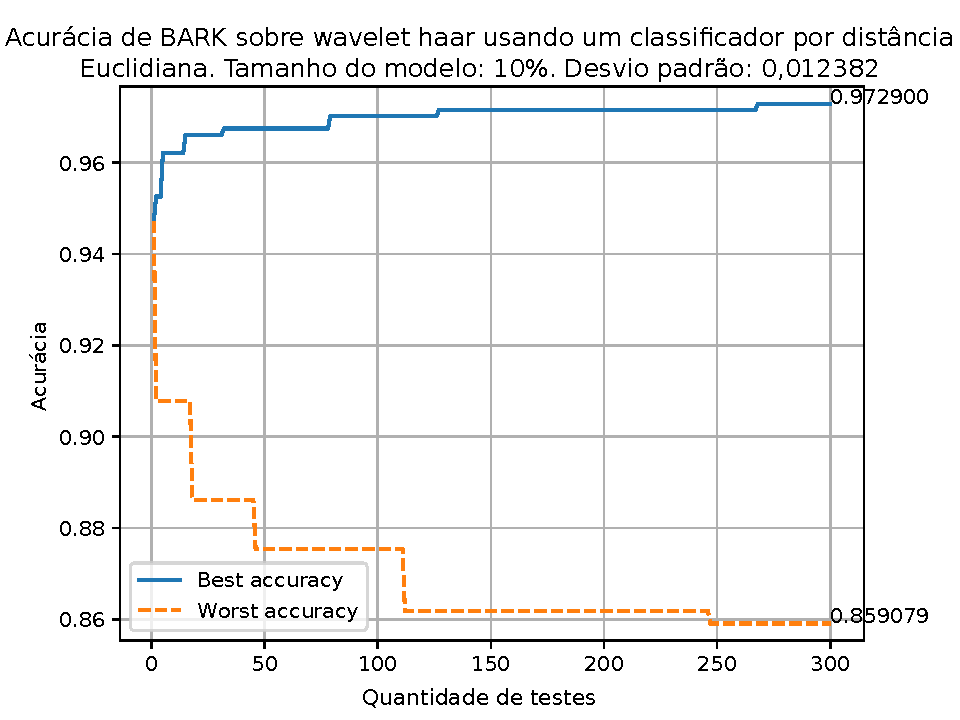
\includegraphics[width=\linewidth]{../monography/images/results/confusionMatrices/classifier_Euclidian_10}
				\caption{Acurácia \textit{X} quantidade de testes - Distância Euclidiana, modelo a 10\%}
			\end{figure}
			
			\column{0.5\textwidth}
			\begin{figure}
				\centering
				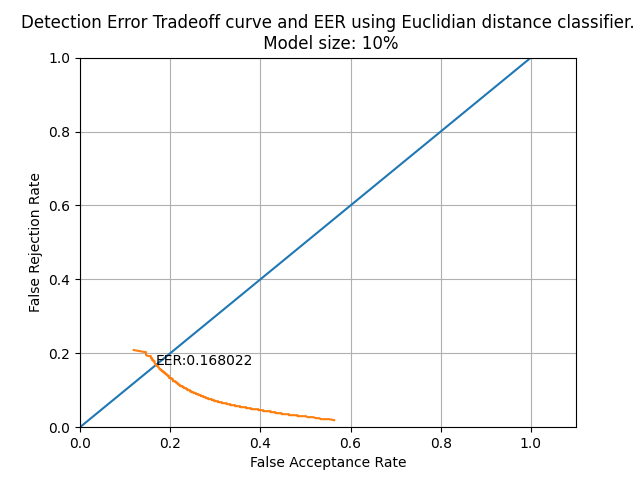
\includegraphics[width=\linewidth]{../monography/images/results/det/DET_for_classifier_Euclidian_10}
				\caption{Curva DET dos resultados de distância Euclidiana, modelo a 10\%}
			\end{figure}
		\end{columns}
	}
	\only<2>{
		\begin{columns}
			\column{0.5\textwidth}
			\begin{figure}
				\centering
				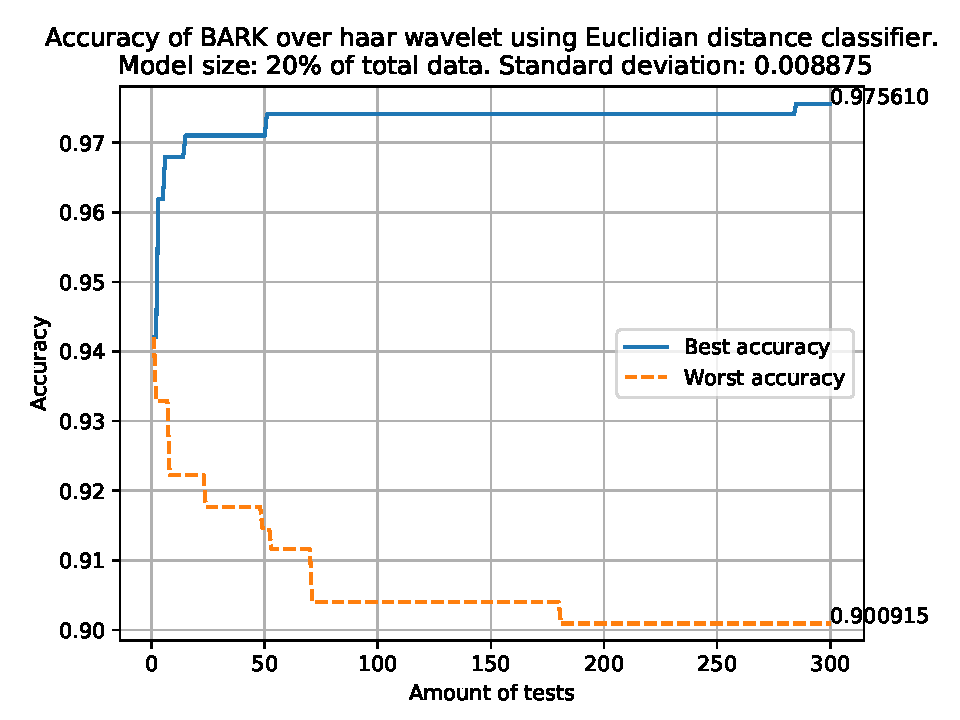
\includegraphics[width=\linewidth]{../monography/images/results/confusionMatrices/classifier_Euclidian_20}
				\caption{Acurácia \textit{X} quantidade de testes - Distância Euclidiana, modelo a 20\%}
			\end{figure}
			
			\column{0.5\textwidth}
			\begin{figure}
				\centering
				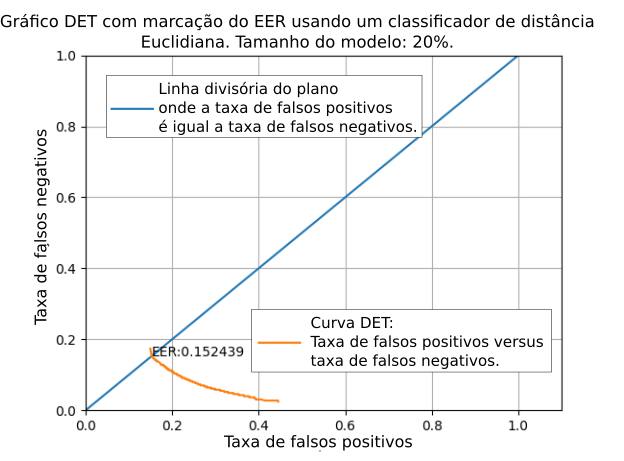
\includegraphics[width=\linewidth]{../monography/images/results/det/DET_for_classifier_Euclidian_20}
				\caption{Curva DET dos resultados de distância Euclidiana, modelo a 20\%}
			\end{figure}
		\end{columns}
	}
	\only<3>{
		\begin{columns}
			\column{0.5\textwidth}
			\begin{figure}
				\centering
				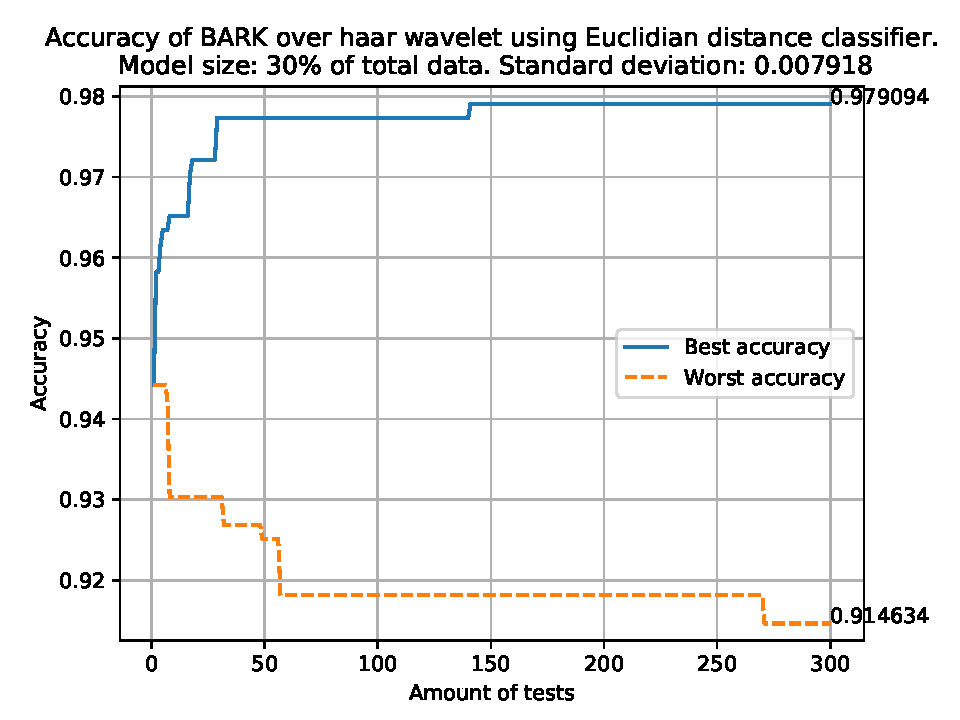
\includegraphics[width=\linewidth]{../monography/images/results/confusionMatrices/classifier_Euclidian_30}
				\caption{Acurácia \textit{X} quantidade de testes - Distância Euclidiana, modelo a 30\%}
			\end{figure}
			
			\column{0.5\textwidth}
			\begin{figure}
				\centering
				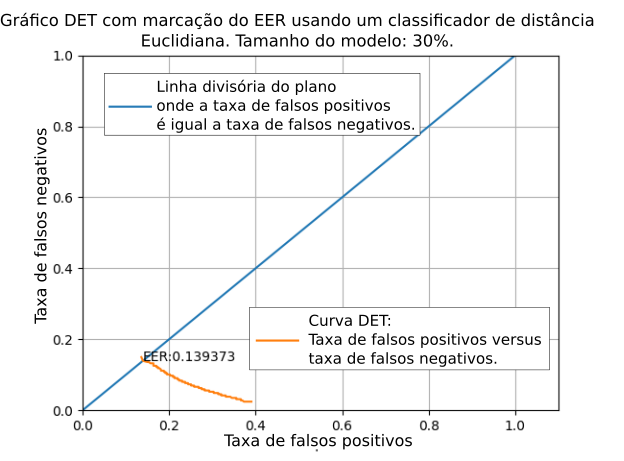
\includegraphics[width=\linewidth]{../monography/images/results/det/DET_for_classifier_Euclidian_30}
				\caption{Curva DET dos resultados de distância Euclidiana, modelo a 30\%}
			\end{figure}
		\end{columns}
	}
	\only<4>{
		\begin{columns}
			\column{0.5\textwidth}
			\begin{figure}
				\centering
				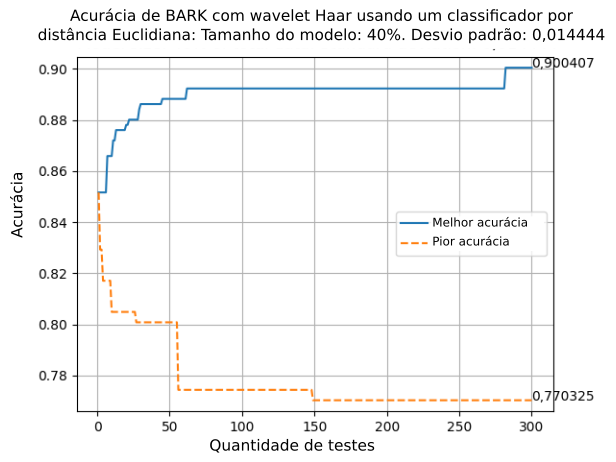
\includegraphics[width=\linewidth]{../monography/images/results/confusionMatrices/classifier_Euclidian_40}
				\caption{Acurácia \textit{X} quantidade de testes - Distância Euclidiana, modelo a 40\%}
			\end{figure}
			
			\column{0.5\textwidth}
			\begin{figure}
				\centering
				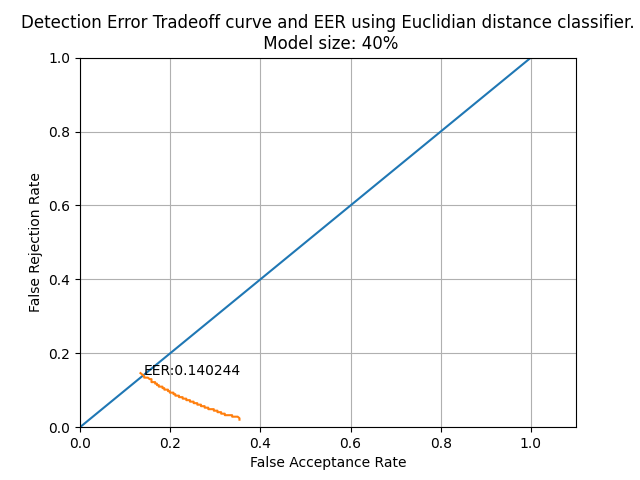
\includegraphics[width=\linewidth]{../monography/images/results/det/DET_for_classifier_Euclidian_40}
				\caption{Curva DET dos resultados de distância Euclidiana, modelo a 40\%}
			\end{figure}
		\end{columns}
	}
	\only<5>{
		\begin{columns}
			\column{0.5\textwidth}
			\begin{figure}
				\centering
				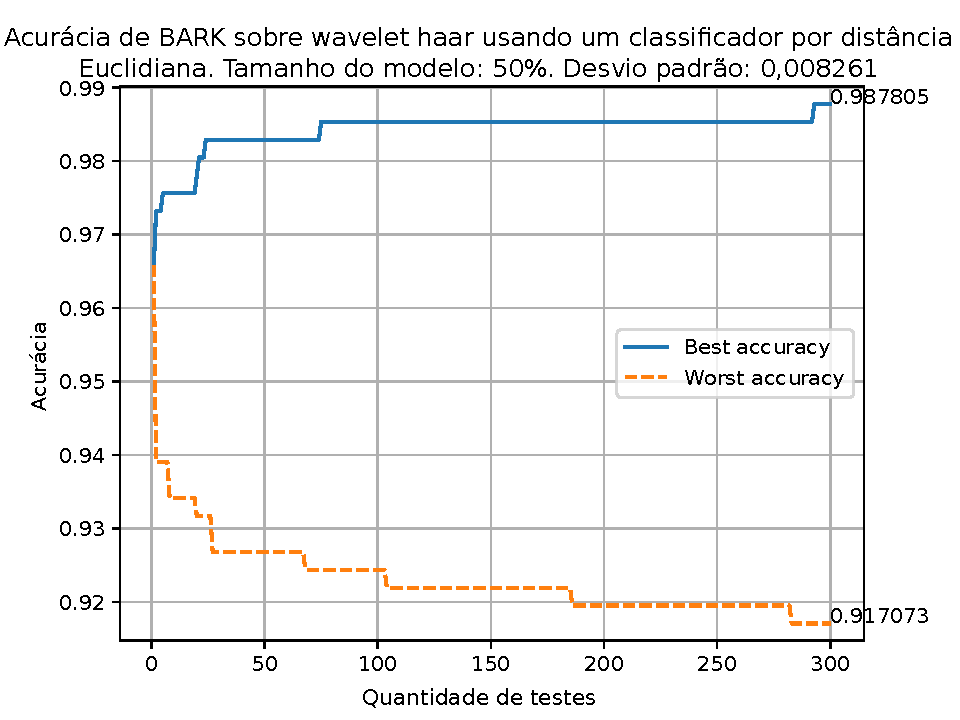
\includegraphics[width=\linewidth]{../monography/images/results/confusionMatrices/classifier_Euclidian_50}
				\caption{Acurácia \textit{X} quantidade de testes - Distância Euclidiana, modelo a 50\%}
			\end{figure}
			
			\column{0.5\textwidth}
			\begin{figure}
				\centering
				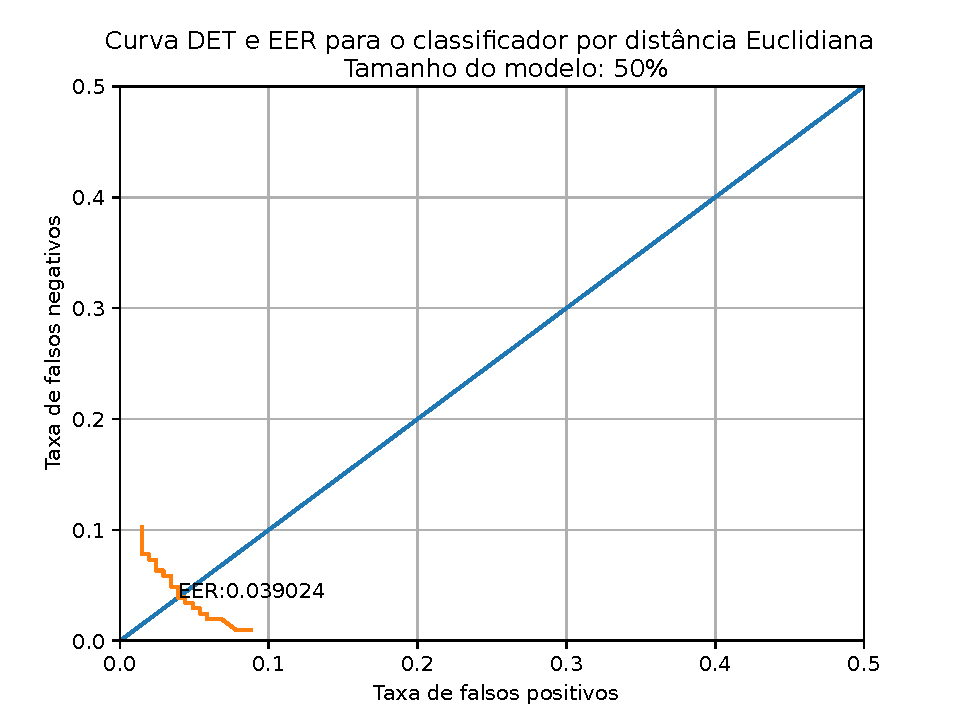
\includegraphics[width=\linewidth]{../monography/images/results/det/DET_for_classifier_Euclidian_50}
				\caption{Curva DET dos resultados de distância Euclidiana, modelo a 50\%}
			\end{figure}
		\end{columns}
	}
\end{frame}

\begin{frame}
	\frametitle{Procedimento 02}
	\framesubtitle{Acurácias e EER para distância Manhattan}
	\only<1>{
		\begin{columns}
			\column{0.5\textwidth}
			\begin{figure}
				\centering
				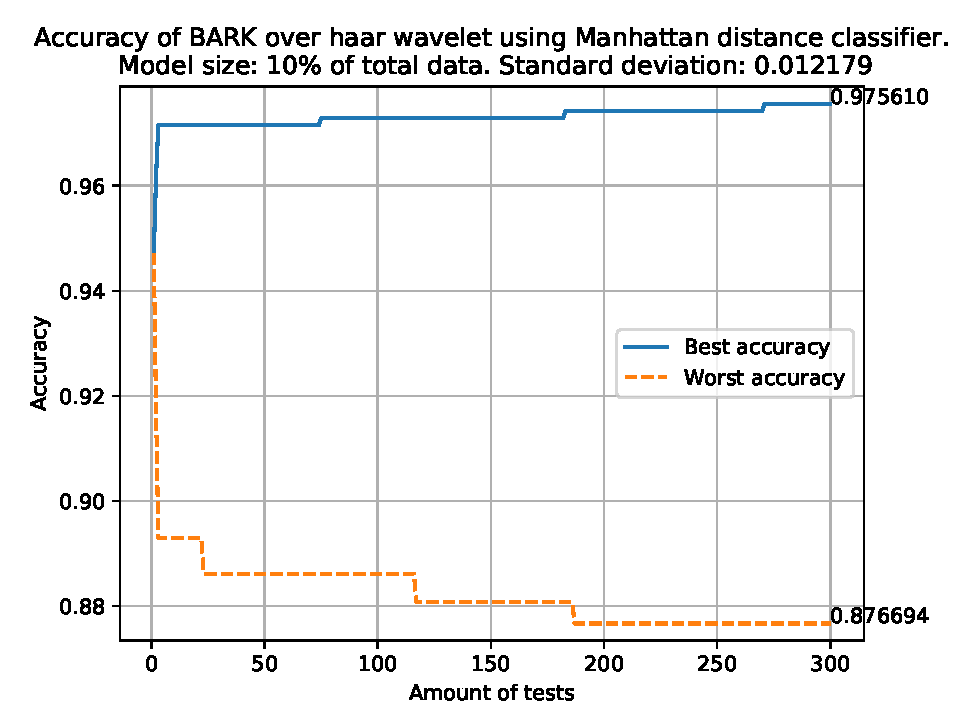
\includegraphics[width=\linewidth]{../monography/images/results/confusionMatrices/classifier_Manhattan_10}
				\caption{Acurácia \textit{X} quantidade de testes - Distância Manhattan, modelo a 10\%}
			\end{figure}
			
			\column{0.5\textwidth}
			\begin{figure}
				\centering
				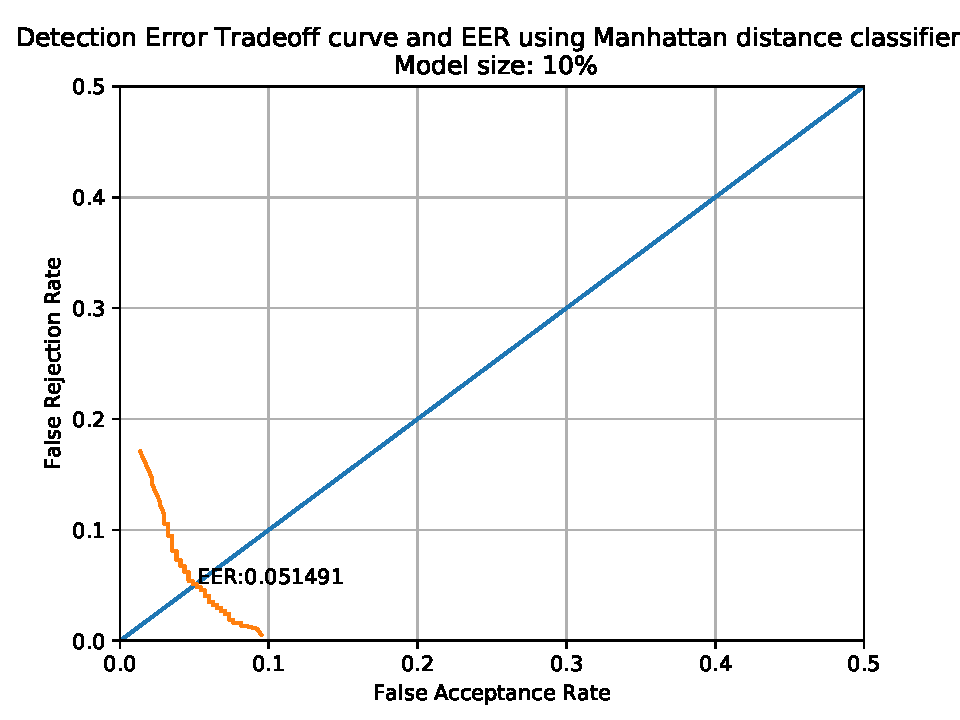
\includegraphics[width=\linewidth]{../monography/images/results/det/DET_for_classifier_Manhattan_10}
				\caption{Curva DET dos resultados de distância Manhattan, modelo a 10\%}
			\end{figure}
		\end{columns}
	}
	\only<2>{
		\begin{columns}
			\column{0.5\textwidth}
			\begin{figure}
				\centering
				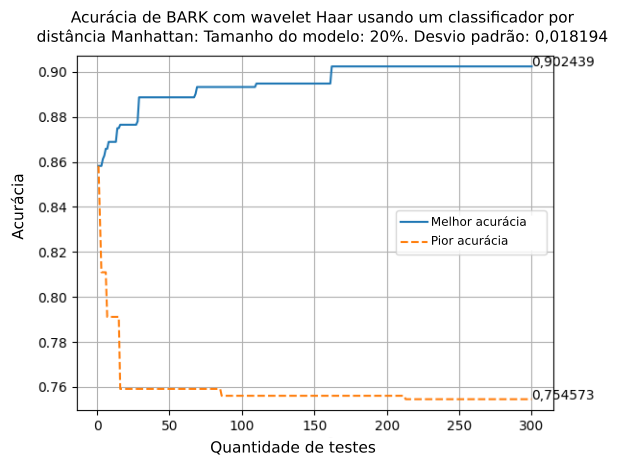
\includegraphics[width=\linewidth]{../monography/images/results/confusionMatrices/classifier_Manhattan_20}
				\caption{Acurácia \textit{X} quantidade de testes - Distância Manhattan, modelo a 20\%}
			\end{figure}
			
			\column{0.5\textwidth}
			\begin{figure}
				\centering
				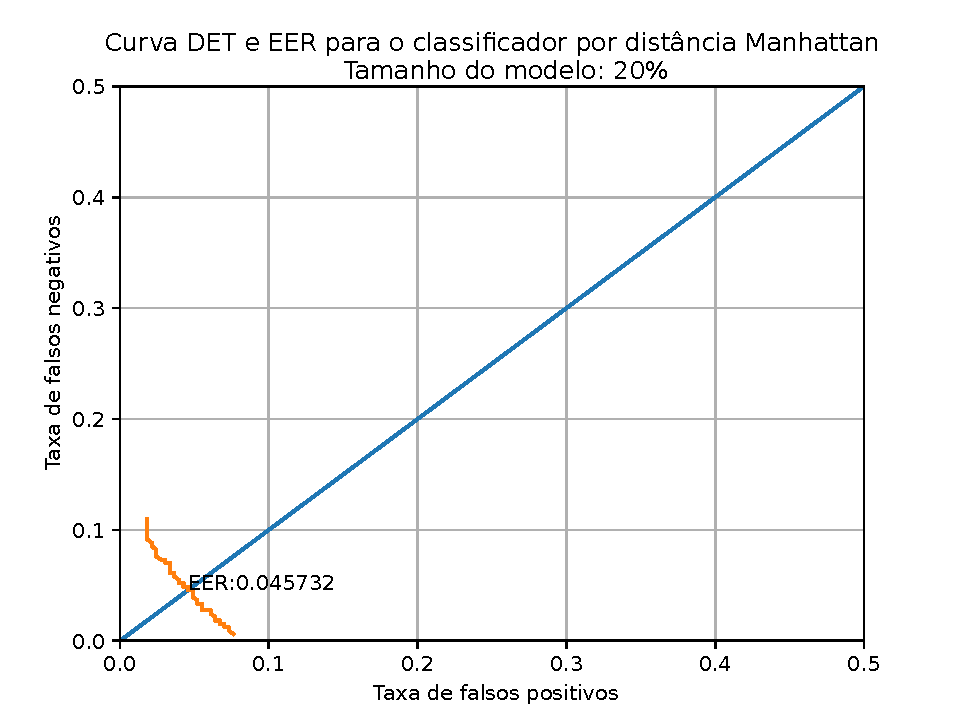
\includegraphics[width=\linewidth]{../monography/images/results/det/DET_for_classifier_Manhattan_20}
				\caption{Curva DET dos resultados de distância Manhattan, modelo a 20\%}
			\end{figure}
		\end{columns}
	}
	\only<3>{
		\begin{columns}
			\column{0.5\textwidth}
			\begin{figure}
				\centering
				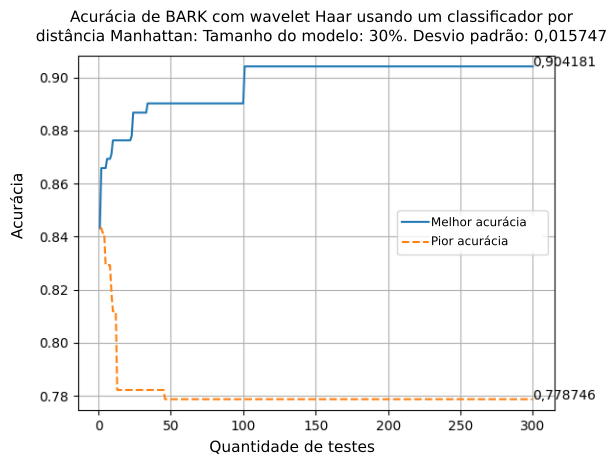
\includegraphics[width=\linewidth]{../monography/images/results/confusionMatrices/classifier_Manhattan_30}
				\caption{Acurácia \textit{X} quantidade de testes - Distância Manhattan, modelo a 30\%}
			\end{figure}
			
			\column{0.5\textwidth}
			\begin{figure}
				\centering
				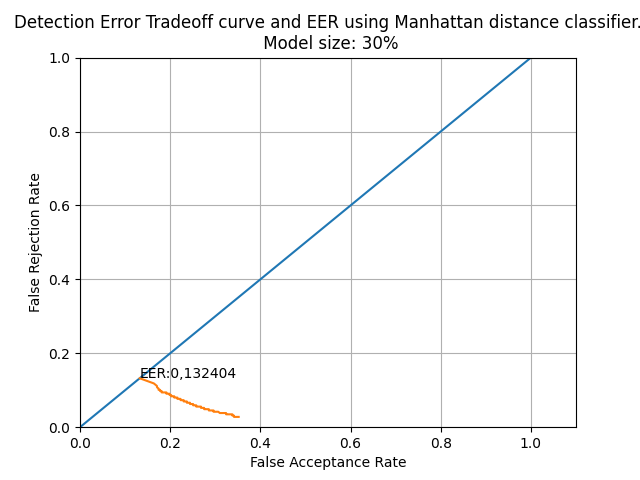
\includegraphics[width=\linewidth]{../monography/images/results/det/DET_for_classifier_Manhattan_30}
				\caption{Curva DET dos resultados de distância Manhattan, modelo a 30\%}
			\end{figure}
		\end{columns}
	}
	\only<4>{
		\begin{columns}
			\column{0.5\textwidth}
			\begin{figure}
				\centering
				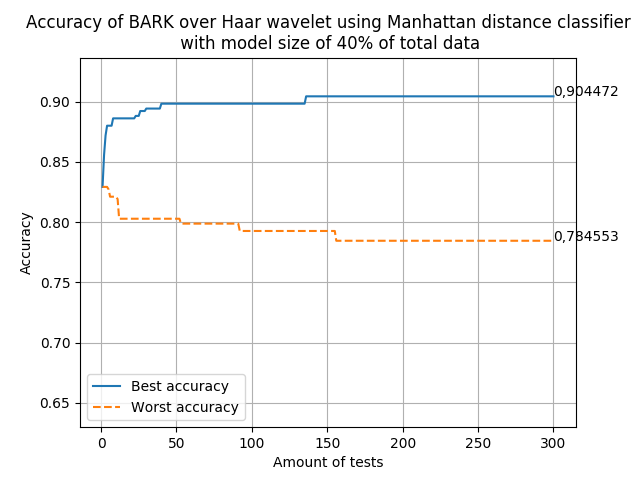
\includegraphics[width=\linewidth]{../monography/images/results/confusionMatrices/classifier_Manhattan_40}
				\caption{Acurácia \textit{X} quantidade de testes - Distância Manhattan, modelo a 40\%}
			\end{figure}
			
			\column{0.5\textwidth}
			\begin{figure}
				\centering
				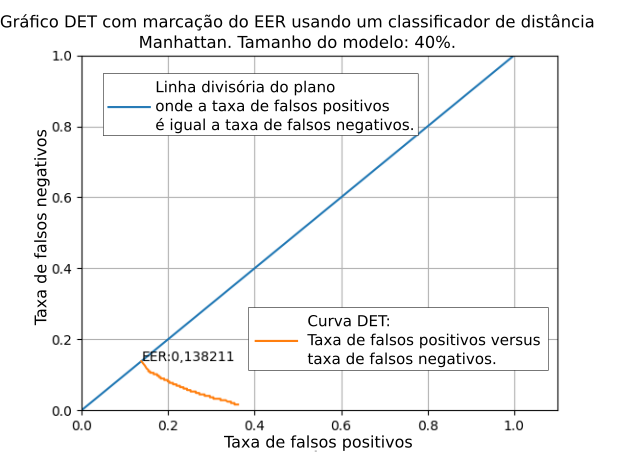
\includegraphics[width=\linewidth]{../monography/images/results/det/DET_for_classifier_Manhattan_40}
				\caption{Curva DET dos resultados de distância Manhattan, modelo a 40\%}
			\end{figure}
		\end{columns}
	}
	\only<5>{
		\begin{columns}
			\column{0.5\textwidth}
			\begin{figure}
				\centering
				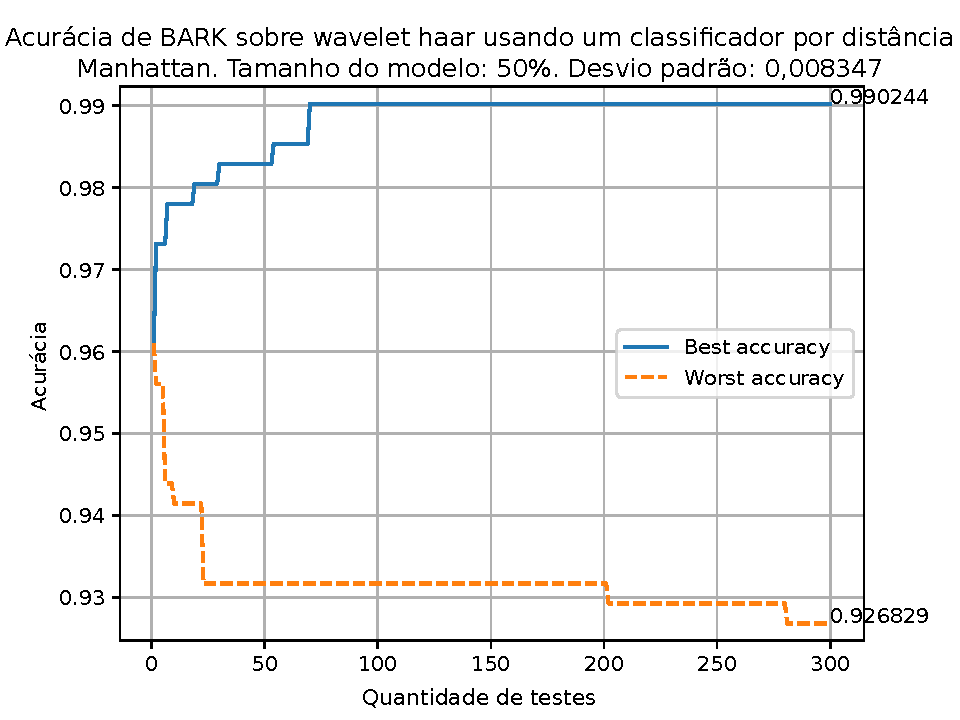
\includegraphics[width=\linewidth]{../monography/images/results/confusionMatrices/classifier_Manhattan_50}
				\caption{Acurácia \textit{X} quantidade de testes - Distância Manhattan, modelo a 50\%}
			\end{figure}
			
			\column{0.5\textwidth}
			\begin{figure}
				\centering
				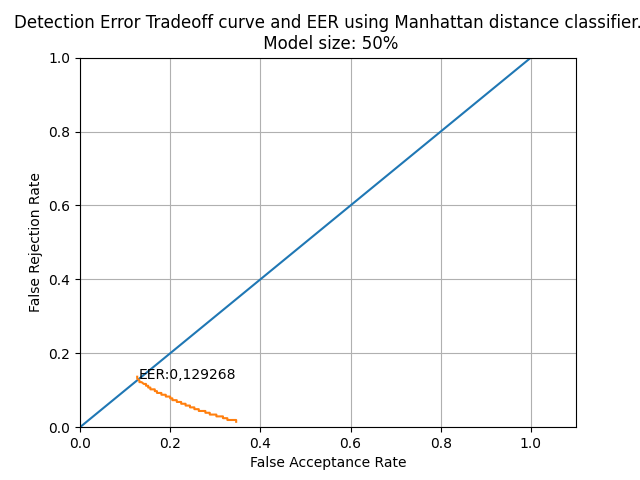
\includegraphics[width=\linewidth]{../monography/images/results/det/DET_for_classifier_Manhattan_50}
				\caption{Curva DET dos resultados de distância Manhattan, modelo a 50\%}
			\end{figure}
		\end{columns}
	}
\end{frame}

\begin{frame}
	\frametitle{Procedimento 02}
		\framesubtitle{Síntese}
		\par Dentre os testes realizados o melhores resultados foram:
		\begin{itemize}
			\item Distância Euclidiana $\rightarrow$ Acurácia: 0,987805 - ERR: 0,039024.
			\item Distância Manhattan $\rightarrow$ Acurácia: 0,990244 - ERR: 0,039024.
		\end{itemize}
\end{frame}